\documentclass[14pt,letterpaper] {article}
\usepackage{enumerate}
\usepackage{algorithm2e}
\usepackage{mcode}
\usepackage{listings}
\usepackage{graphicx}
\usepackage{epsf}

\author{Zhengwu Zhang}
\title{Homework 5}

\begin{document} 
\maketitle
\newpage

\subsection{Problem 1}
\subsubsection{(a)}
\begin{figure}
\begin{center}
\includegraphics[width=5.4in, height=2.4in]{plotx.eps}
\caption{Answer of part (a), Plot of {$x_i$}}
\end{center}
\end{figure}

\begin{figure}
\begin{center}
\includegraphics[width=5.4in, height=2.2in]{ploty.eps}
\caption{Answer of part (a), Plot of {$y_i$}}
\end{center}
\end{figure}

\subsubsection{(b)}

The estimation of A,H,W,Q with $x_i$,$y_i$ is: \\

\begin{lstlisting}

K>> Ah

Ah =

    0.9389    0.1146   -0.1880
   -0.3236    0.8125    0.0553
    0.2476    0.1298    0.9094

K>> Qh

Qh =

    0.5121    0.0211
    0.0211    0.5435

K>> Hh

Hh =

    0.9796    0.4821    0.2033
    0.4827    0.9973    0.0990

K>> Wh

Wh =

    0.8637   -0.0313    0.0197
   -0.0313    1.0675   -0.0595
    0.0197   -0.0595    1.0448
    
    K>> norm(Ah-A)/norm(A)

ans =

    0.0757

K>> norm(Qh-Q)/norm(Q)

ans =

    0.1081

K>> norm(Hh-H)/norm(H)

ans =

    0.0207

K>> norm(Wh-W)/norm(W)

ans =

    0.1416

\end{lstlisting}

\subsubsection{(c)}

\begin{figure}
\begin{center}
\includegraphics[width=5.4in, height=2.4in]{partc.eps}
\caption{Answer of part (c), Plot of true data and estiamtion}
\end{center}
\end{figure}


We could not have the same accuracy for the third components. The reasons is: (1) $x$ is a three dimensional data and $y$ is a two dimensional data, 
we are using the two dimensional data to estimate three dimensional data, there mush one dimension that now correct enough. (2) From the matrix H, we can get that
$y_1=x_1+0.5*x_2+0.2x_3$, and $y_2=0.5*x_1+x_2+0.1x_3$, we can see that $x_1$ are dominated by $y_1$, similar as $x_2$, but $x_3$ is just like a noise. So it could not
be estimated well enough. 
\subsubsection{(d)}

\begin{lstlisting}
>>  R2m

R2m =

    0.8323
    0.9501
    0.4549

>> R2p

R2p =

    0.6015
    0.8553
    0.4364

\end{lstlisting}

Compare the results: We can see that the $R^2$-Error for the filtering estimation is higher than the prediction estimation.  Bigger $R^2$ means 
higher estimation eccuracy.  

\subsection{Problem 2}
If we change $Q=50I_2$, the $R^2$-Error we get is:

\begin{lstlisting}
R2m =

    0.1201
    0.3227
    0.1853

>> R2p

R2p =

    0.0907
    0.2620
    0.1875
\end{lstlisting}

We can see that the estimation accuracy decrease significantly. However, the $R^2$ in the filtering estimation have no significant different with
the ones in prediction estimation. 

\subsection{Problem 3}

\begin{figure}
\begin{center}
\begin{tabular}{cc}
\includegraphics[width=2.4in, height=1.4in]{3plotx.eps}&
\includegraphics[width=2.4in, height=1.4in]{3ploty.eps}\\
(a) & (b) \\
\end{tabular}
\caption{Answer of problem 3 (a) plot of $x$ (b) plot of $y$}
\end{center}
\end{figure}

We can see that the process is very unstable. The reason is that the eigenvalues of the Matrix $A$ is greater than 1.

\begin{lstlisting}
K>> eig(A)

ans =

    1.2091
    0.7812
    0.4097

\end{lstlisting}

Because 
$$
X_k=A*X_{k-1}+W_k=A^{k-1}*X_1+W_k
$$ 

So if one of the eigenvalue of A greater than 1, $X_k$ are going to be very big as k increase. 

\end{document}